\chapter{Specifikacija programske potpore}
		
	\section{Funkcionalni zahtjevi}
			
			\noindent \textbf{Dionici:}
			
			\begin{packed_enum}
				
				\item Neregistrirani korisnik
				\item Korisnik
				\begin{packed_enum}
					\item Vlasnik pasa
					\item Čuvar pasa
				\end{packed_enum}
				\item Administrator 				
				\item Razvojni tim
				
			\end{packed_enum}
			
			\noindent \textbf{Aktori i njihovi funkcionalni zahtjevi:}
			
			
			\begin{packed_enum}
				\item  \underbar{Neregistrirani korisnik (inicijator) može:}
				
				\begin{packed_enum}
					
					\item Na početnoj stranici pregledavati zahtjeve i oglase
					\item Odabrati željeni zahtjev/oglas i vidjeti pojedinosti tog zahtjeva/oglasa (pasmina, dob, lokacija itd.)
					\item Registrirati se u sustav, stvoriti novi korisnički račun za koji mu trebaju ime, prezime, korisničko ime, e-mail adresa, lozinka, broj telefona i uloga.
				\end{packed_enum}
				
				\item  \underbar{Korisnik (inicijator) može:}
				
				\begin{packed_enum}
					
					\item Pregledavati i mijenjati osobne podatke
					\item Odjaviti se s korisničkog računa i prijaviti se nekim drugim računom
					\item Imati ulogu vlasnika pasa:
					\begin{packed_enum}
						\item Stvarati novi zahtjev za čuvanje pasa
						\item Stupiti u kontakt s potencijalnim čuvarom pasa
						\item Spremiti podatke o svom psu
						\item Ocjenjivati uslugu čuvara
						\item Pregledavati vlastite zahtjeve
					\end{packed_enum}
					\item Imati ulogu čuvara pasa:
					\begin{packed_enum}
						\item Stvarati novi oglas za čuvanje pasa
						\item Stupiti u kontakt s vlasnikom pasa
						\item Termine čuvanja pasa spremati u svoj kalendar
						\item Ocjenjivati ponašanje psa
						\item Pregledavati vlastite oglase
					\end{packed_enum}
				\end{packed_enum}
			
				\item \underbar{Administrator (inicijator) može:}
				\begin{packed_enum}
					\item Obavljati sve funkcionalnosti korisnika
					\item Dodijeliti administratorsku ulogu drugim korisnicima
					\item Odobriti ili odbaciti zahtjev/oglas
					\item Blokirati korisnika koji narušava pravila sustava
				\end{packed_enum}
			
				\item \underbar{Baza podataka (sudionik) može:}
				\begin{packed_enum}
					\item Pohraniti sve podatke o korisnicima i njihovim ulogama
					\item Pohraniti sve podatke o psima
					\item Pohraniti sve podatke o provedenim oglasima i zahtjevima
					\item Pohraniti podatke o mogućima aktivnostima sa psima
				\end{packed_enum}
			
			\end{packed_enum}
			
			\eject 
			
			
				
			\subsection{Obrasci uporabe}
				
				\subsubsection{Opis obrazaca uporabe}					

					\noindent \underbar{\textbf{UC01 - Pregledavanje zahtjeva/oglasa}}
					\begin{packed_item}
	
						\item \textbf{Glavni sudionik: } Neregistrirani korisnik 
						\item  \textbf{Cilj:} Pregledati ponuđene oglase i zahtjeve
						\item  \textbf{Sudionici:} Baza podataka 
						\item  \textbf{Preduvjet:} -
						\item  \textbf{Opis osnovnog tijeka:}
						
						\item[] \begin{packed_enum}
	
							\item Prilikom učitavanja aplikacije prikazuje se lista zahtjeva i lista oglasa
							\item Klikom na zahtjev/oglas prikazuju se dodatne informacije o tom zahtjevu/oglasu
				
						\end{packed_enum}
					\end{packed_item}
					
					\noindent \underbar{\textbf{UC02 - Registracija}}
					\begin{packed_item}
						
						\item \textbf{Glavni sudionik: } Neregistrirani korisnik 
						\item  \textbf{Cilj:} Stvoriti korisnički račun za korištenje svih funkcionalnosti aplikacije
						\item  \textbf{Sudionici:} Baza podataka 
						\item  \textbf{Preduvjet:} -
						\item  \textbf{Opis osnovnog tijeka:}
						
						\item[] \begin{packed_enum}
							
							\item Korisnik pristupa padajućem izborniku i odabire opciju za registraciju 
							\item Korisnik unosi korisničke podatke potrebne za registraciju i potvrđuje upis
							\item Korisnik dobiva povratnu informaciju o uspješnoj registraciji i preusmjerava se na početnu stranicu
							\item Korisnik se upisuje u bazu podataka
							
						\end{packed_enum}
						
						\item  \textbf{Opis mogućih odstupanja:}
						
						\item[] \begin{packed_item}
	
							\item[2.a] Odabir već zauzetog korisničkog imena i/ili e-maila, unos korisničkih podataka u neispravnom formatu, nepodudaranje lozinki 
							\item[] \begin{packed_enum}
								
								\item Sustav obavještava korisnika o neuspjelom upisu i vraća ga na stranicu za registraciju 
								\item Korisnik mijenja potrebne podatke te završava unos ili odustaje od registracije
								
							\end{packed_enum}
							
							
						\end{packed_item}
					\end{packed_item}
				
					\noindent \underbar{\textbf{UC03 - Prijava}}
					\begin{packed_item}
					
						\item \textbf{Glavni sudionik: } Korisnik 
						\item  \textbf{Cilj:} Dobivanje pristupa svim funkcionalnostima aplikacije
						\item  \textbf{Sudionici:} Baza podataka 
						\item  \textbf{Preduvjet:} Korisnik je pohranjen u bazu podataka
						\item  \textbf{Opis osnovnog tijeka:}
					
						\item[] \begin{packed_enum}
						
							\item Korisnik pristupa padajućem izborniku i odabire opciju za prijavu 
							\item Korisnik unosi korisničko ime i lozinku te potvrđuje upis
							\item Korisnik dobiva povratnu informaciju o uspješnoj prijavi i preusmjerava se na početnu stranicu
						
						\end{packed_enum}
					
						\item  \textbf{Opis mogućih odstupanja:}
					
						\item[] \begin{packed_item}
						
							\item[2.a] Neispravni unos korisničkog imena i/ili lozinke  
							\item[] \begin{packed_enum}
							
								\item Sustav obavještava korisnika o neuspjelom upisu i vraća ga na stranicu za prijavu  
								\item Korisnik unosi ispravne podatke za prijavu ili odustaje od prijave
							
							\end{packed_enum}
						\end{packed_item}
					\end{packed_item}
				
					\noindent \underbar{\textbf{UC04 - Odjava iz sustava}}
					\begin{packed_item}
						
						\item \textbf{Glavni sudionik: } Korisnik 
						\item  \textbf{Cilj:} Odjaviti se iz sustava
						\item  \textbf{Sudionici:} Baza podataka 
						\item  \textbf{Preduvjet:} Korisnik je prijavljen
						\item  \textbf{Opis osnovnog tijeka:}
						
						\item[] \begin{packed_enum}
							
							\item Korisnik pristupa padajućem izborniku i odabire opciju "Odjava" 
							\item Aplikacija korisnika odjavljuje s trenutnog korisničkog računa
							\item Korisnik se preusmjerava na početnu stranicu gdje mu se pruža lista zahtjeva i oglasa
							
						\end{packed_enum}
					\end{packed_item}
				
					\noindent \underbar{\textbf{UC05 - Pregled osobnih podataka}}
					\begin{packed_item}
						
						\item \textbf{Glavni sudionik: } Korisnik 
						\item  \textbf{Cilj:} Pregledati osobne podatke
						\item  \textbf{Sudionici:} Baza podataka 
						\item  \textbf{Preduvjet:} Korisnik je prijavljen
						\item  \textbf{Opis osnovnog tijeka:}
						
						\item[] \begin{packed_enum}
							
							\item Korisnik pristupa padajućem izborniku i odabire opciju "Moj račun" 
							\item Aplikacija prikazuje osobne podatke korisnika
							
						\end{packed_enum}
					\end{packed_item}
					
					\iffalse
					\noindent \underbar{\textbf{UC06 - Promjena osobnih podataka}}
					\begin{packed_item}
						
						\item \textbf{Glavni sudionik: } Korisnik 
						\item  \textbf{Cilj:} Promijeniti osobne podatke
						\item  \textbf{Sudionici:} Baza podataka 
						\item  \textbf{Preduvjet:} Korisnik je prijavljen
						\item  \textbf{Opis osnovnog tijeka:}
						
						\item[] \begin{packed_enum}
							
							\item Korisnik pristupa padajućem izborniku i odabire opciju „Moj račun“  
							\item Korisnik odabire opciju uredi osobne podatke
							\item Korisnik mijenja osobne podatke
							\item Korisnik sprema promjene
							\item Baza podataka se ažurira
							
						\end{packed_enum}
						
						\item  \textbf{Opis mogućih odstupanja:}
						
						\item[] \begin{packed_item}
							
							\item[4.a] Korisnik promijeni svoje osobne podatke, ali ne odabere opciju ”Spremi” 
							\item[] \begin{packed_enum}
								
								\item Promjene se ne spremaju
								
							\end{packed_enum}
						\end{packed_item}
					\end{packed_item}
					\fi
					
					\noindent \underbar{\textbf{UC06 – Dodavanje pasa}}
					\begin{packed_item}
						
						\item \textbf{Glavni sudionik: } Korisnik (vlasnik pasa)
						\item  \textbf{Cilj:} Dodavanje pasa na web stranicu
						\item  \textbf{Sudionici:} Baza podataka 
						\item  \textbf{Preduvjet:} Korisnik je prijavljen, korisnik ima ulogu vlasnika pasa
						\item  \textbf{Opis osnovnog tijeka:}
						
						\item[] \begin{packed_enum}
							
							\item Korisnik na padajućem izborniku odabire opciju "Moji psi" 
							\item Korisnik na stranici s prikazom vlastitih pasa odabire gumb "Dodaj psa"
							\item Korisnik ispunjava osobne podatke o psu
							\item Korisnik odabire gumb "Spremi"
							\item Podaci o psu se spremaju u sustav
							
						\end{packed_enum}
					
				
						\item  \textbf{Opis mogućih odstupanja:}
		
						\item[] \begin{packed_item}
	
							\item[4.a] Korisnik zaboravlja pritisnuti gumb "Spremi"
							\item[] \begin{packed_enum}
								\item Podaci o psu se ne spremaju u sustav
							\end{packed_enum}
						\end{packed_item}
					\end{packed_item}
					
					\noindent \underbar{\textbf{UC07 – Pregledavanje tuđih zahtjeva}}
					\begin{packed_item}
						
						\item \textbf{Glavni sudionik: } Korisnik 
						\item  \textbf{Cilj:} Pronalaženje najprikladnijeg zahtjeva
						\item  \textbf{Sudionici:} Baza podataka 
						\item  \textbf{Preduvjet:} Korisnik je prijavljen, korisnik ima ulogu čuvara
						\item  \textbf{Opis osnovnog tijeka:}
						
						\item[] \begin{packed_enum}
							
							\item Korisnik na početnoj stranici prolazi kroz listu tuđih zahtjeva 
							\item Korisnik odabire odgovarajući zahtjev
							\item Korisnik pregledava dodatne podatke o tom zahtjevu
							
						\end{packed_enum}
					\end{packed_item}
				
					\noindent \underbar{\textbf{UC08 – Pregledavanje tuđih oglasa}}
					\begin{packed_item}
						
						\item \textbf{Glavni sudionik: } Korisnik 
						\item  \textbf{Cilj:} Pronalaženje najprikladnijeg oglasa
						\item  \textbf{Sudionici:} Baza podataka 
						\item  \textbf{Preduvjet:} Korisnik je prijavljen, korisnik ima ulogu vlasnika
						\item  \textbf{Opis osnovnog tijeka:}
						
						\item[] \begin{packed_enum}
							
							\item Korisnik na početnoj stranici prolazi kroz listu tuđih oglasa  
							\item Korisnik odabire odgovarajući oglas
							\item Korisnik pregledava dodatne podatke o tom oglasu
							
						\end{packed_enum}
					\end{packed_item}

					\noindent \underbar{\textbf{UC09 – Pregledavanje vlastitih zahtjeva}}
					\begin{packed_item}
						
						\item \textbf{Glavni sudionik: } Korisnik (vlasnik pasa)
						\item  \textbf{Cilj:} Pregledavanje svojih kreiranih zahtjeva
						\item  \textbf{Sudionici:} Baza podataka 
						\item  \textbf{Preduvjet:} Korisnik je prijavljen, korisnik ima ulogu vlasnika
						\item  \textbf{Opis osnovnog tijeka:}
						
						\item[] \begin{packed_enum}
							
							\item Korisnik pristupa padajućem izborniku i odabire opciju "Moji zahtjevi"  
							\item Korisniku se prikazuje lista zahtjeva
							
						\end{packed_enum}
					
						\item  \textbf{Opis mogućih odstupanja:}
						
						\item[] \begin{packed_item}
							
							\item[2.a] Korisnik nema kreiranih zahtjeva
							\item[] \begin{packed_enum}
								
								\item Korisniku se prikazuje prikladna poruka
								
							\end{packed_enum}
						\end{packed_item}
					\end{packed_item}	
				
					\noindent \underbar{\textbf{UC10 – Pregledavanje vlastitih oglasa}}
					\begin{packed_item}
						
						\item \textbf{Glavni sudionik: } Korisnik (čuvar pasa)
						\item  \textbf{Cilj:} Pregledavanje svojih kreiranih oglasa
						\item  \textbf{Sudionici:} Baza podataka 
						\item  \textbf{Preduvjet:} Korisnik je prijavljen, korisnik ima ulogu čuvara
						\item  \textbf{Opis osnovnog tijeka:}
						
						\item[] \begin{packed_enum}
							
							\item Korisnik pristupa padajućem izborniku i odabire opciju "Moji oglasi"  
							\item Korisniku se prikazuje lista oglasa
							
						\end{packed_enum}
						
						\item  \textbf{Opis mogućih odstupanja:}
						
						\item[] \begin{packed_item}
							
							\item[2.a] Korisnik nema kreiranih oglasa
							\item[] \begin{packed_enum}
								
								\item Korisniku se prikazuje prikladna poruka
								
							\end{packed_enum}
						\end{packed_item}
					\end{packed_item}	
				
					\noindent \underbar{\textbf{UC11 – Kreiranje novog zahtjeva}}
					\begin{packed_item}
						
						\item \textbf{Glavni sudionik: } Korisnik (vlasnik pasa)
						\item  \textbf{Cilj:} Objavljivanje novog zahtjeva za čuvanje pasa
						\item  \textbf{Sudionici:} Baza podataka, administrator
						\item  \textbf{Preduvjet:} Korisnik je prijavljen, korisnik ima ulogu vlasnika
						\item  \textbf{Opis osnovnog tijeka:}
						
						\item[] \begin{packed_enum}
							
							\item Korisnik na početnoj stranici odabire opciju za kreiranje novog zahtjeva   
							\item Korisniku se otvara stranica za kreiranje zahtjeva
							\item Korisnik unosi sve tražene podatke za kreiranje zahtjeva (pasmina, dob, period čuvanja itd.)
							\item Korisnik odabire opciju za objavljivanje zahtjeva
							\item Zahtjev se šalje administratoru na uvid
							
						\end{packed_enum}
						
						\item  \textbf{Opis mogućih odstupanja:}
						
						\item[] \begin{packed_item}
							
							\item[4.a] Korisnik nije ispravno unio sve podatke
							\item[] \begin{packed_enum}
								
								\item Korisnika se ponovno vraća na stranicu za kreiranje zahtjeva s odgovarajućom porukom o greški 
								
							\end{packed_enum}
						\end{packed_item}
					\end{packed_item}		
				
					\noindent \underbar{\textbf{UC12 – Kreiranje novog oglasa}}
					\begin{packed_item}
						
						\item \textbf{Glavni sudionik: } Korisnik (čuvar pasa)
						\item  \textbf{Cilj:} Objavljivanje novog oglasa  za čuvanje pasa
						\item  \textbf{Sudionici:} Baza podataka, administrator
						\item  \textbf{Preduvjet:} Korisnik je prijavljen, korisnik ima ulogu čuvara
						\item  \textbf{Opis osnovnog tijeka:}
						
						\item[] \begin{packed_enum}
							
							\item Korisnik na početnoj stranici odabire opciju za kreiranje novog oglasa     
							\item Korisniku se otvara stranica za kreiranje oglasa  
							\item Korisnik unosi sve tražene podatke za kreiranje oglasa   (preferirana pasmina, preferirana dob, period čuvanja itd.)
							\item Korisnik odabire opciju za objavljivanje oglasa
							\item Oglas se šalje administratoru na uvid
							
						\end{packed_enum}
						
						\item  \textbf{Opis mogućih odstupanja:}
						
						\item[] \begin{packed_item}
							
							\item[4.a] Korisnik nije ispravno unio sve podatke
							\item[] \begin{packed_enum}
								
								\item Korisnika se ponovno vraća na stranicu za kreiranje oglasa s odgovarajućom porukom o greški 
								
							\end{packed_enum}
						\end{packed_item}
					\end{packed_item}	
				
					\noindent \underbar{\textbf{UC13 – Pronalaženje najboljeg odabira čuvara pasa}}
					\begin{packed_item}
						
						\item \textbf{Glavni sudionik: } Korisnik (vlasnik pasa)
						\item  \textbf{Cilj:} Pronalaženje najprikladnijeg čuvara pasa
						\item  \textbf{Sudionici:} Baza podataka, korisnik (čuvar pasa)
						\item  \textbf{Preduvjet:} Korisnikov zahtjev je potvrđen od administratora
						\item  \textbf{Opis osnovnog tijeka:}
						
						\item[] \begin{packed_enum}
							
							\item Korisnik pristupa padajućem izborniku i odabire opciju "Moji zahtjevi"    
							\item Korisnik na listi zahtjeva pokraj željenog zahtjeva pritišće gumb "Pronalaženje najboljeg odabira"  
							\item Korisnik (čuvar) dobiva obavijest sa najpogodnijim zahtjevom
							\item Korisnici prihvaćaju odabir
							\item Korisnici razmjenjuju detalje
							
						\end{packed_enum}
					
						\item  \textbf{Opis mogućih odstupanja:}
			
							\item[] \begin{packed_item}
							\item[4.a] Korisnik (vlasnik) odbija zahtjev
							\item[] \begin{packed_enum}
			
								\item Daljnja suradnja između korisnika nije moguća
			
							\end{packed_enum}
						
							\item[4.b] Korisnik (čuvar) odbija zahtjev
							\item[] \begin{packed_enum}
								
								\item Daljnja suradnja između korisnika nije moguća
								
							\end{packed_enum}
						\end{packed_item}
					\end{packed_item}	
				
					\noindent \underbar{\textbf{UC14 – Pronalaženje najboljeg odabira vlasnika pasa}}
					\begin{packed_item}
						
						\item \textbf{Glavni sudionik: } Korisnik (čuvar pasa)
						\item  \textbf{Cilj:} Pronalaženje najprikladnijeg psa za čuvanje
						\item  \textbf{Sudionici:} Baza podataka, korisnik (vlasnik pasa)
						\item  \textbf{Preduvjet:} Korisnikov oglas je potvrđen od administratora
						\item  \textbf{Opis osnovnog tijeka:}
						
						\item[] \begin{packed_enum}
							
							\item Korisnik pristupa padajućem izborniku i odabire opciju "Moji oglasi"    
							\item Korisnik na listi oglasa pokraj željenog oglasa pritišće gumb "Pronalaženje najboljeg odabira"  
							\item Korisnik (vlasnik) dobiva obavijest sa najboljim odabirom
							\item Korisnici prihvaćaju odabir
							\item Korisnici razmjenjuju detalje
							
						\end{packed_enum}
						
						\item  \textbf{Opis mogućih odstupanja:}
						
						\item[] \begin{packed_item}
							
							\item[4.a] Korisnik (vlasnik) odbija zahtjev
							\item[] \begin{packed_enum}
								
								\item Daljnja suradnja između korisnika nije moguća
								
							\end{packed_enum}
							\item[4.b] Korisnik (čuvar) odbija zahtjev
							\item[] \begin{packed_enum}
								
								\item Daljnja suradnja između korisnika nije moguća
								
							\end{packed_enum}
						\end{packed_item}
					\end{packed_item}	
				
					\noindent \underbar{\textbf{UC15 – Javljanje na oglas}}
					\begin{packed_item}
						
						\item \textbf{Glavni sudionik: } Korisnik (vlasnik pasa)
						\item  \textbf{Cilj:} Pronalaženje najprikladnijeg čuvara pasa
						\item  \textbf{Sudionici:} Baza podataka, korisnik (čuvar pasa)
						\item  \textbf{Preduvjet:} Korisnikov zahtjev je potvrđen od administratora
						\item  \textbf{Opis osnovnog tijeka:}
						
						\item[] \begin{packed_enum}
							
							\item Korisnik na početnoj stranici prolazi kroz listu tuđih oglasa   
							\item Korisnik odabire odgovarajući oglas
							\item Korisnik pregledava dodatne podatke o tom oglasu
							\item Korisnik odabire oglas 
							\item Korisniku (čuvaru) se šalje obavijest o odabiru
							\item Korisnik (čuvar) prihvaća odabir
							\item Korisnici razmjenjuju detalje
							
						\end{packed_enum}
						
						\item  \textbf{Opis mogućih odstupanja:}
						
						\item[] \begin{packed_item}
							
							\item[4.a] Korisniku se ne sviđa oglas (ne odabire oglas)
							\item[] \begin{packed_enum}
								
								\item Korisnik se vraća na početnu listu
								\item Korisnik nastavlja s pretraživanjem
								
							\end{packed_enum}
						
							\item[6.a] Korisnik (čuvar) odbija zahtjev 
							\item[] \begin{packed_enum}
								
								\item Daljnja suradnja između korisnika nije moguća
								
							\end{packed_enum}
						\end{packed_item}
					\end{packed_item}	

					\noindent \underbar{\textbf{UC16 – Javljanje na zahtjev}}
					\begin{packed_item}
						
						\item \textbf{Glavni sudionik: } Korisnik (čuvar pasa)
						\item  \textbf{Cilj:} Pronalaženje najprikladnijeg psa za čuvanje
						\item  \textbf{Sudionici:} Baza podataka, korisnik (vlasnik pasa)
						\item  \textbf{Preduvjet:} Korisnikov oglas je potvrđen od administratora
						\item  \textbf{Opis osnovnog tijeka:}
						
						\item[] \begin{packed_enum}
							
							\item Korisnik na početnoj stranici prolazi kroz listu tuđih zahtjeva   
							\item Korisnik odabire odgovarajući zahtjev
							\item Korisnik pregledava dodatne podatke o tom zahtjevu
							\item Korisnik odabire zahtjev 
							\item Korisniku (vlasniku) se šalje obavijest o odabiru
							\item Korisnik (vlasnik) prihvaća odabir
							\item Korisnici razmjenjuju detalje
							
						\end{packed_enum}
						
						\item  \textbf{Opis mogućih odstupanja:}
						
						\item[] \begin{packed_item}
							
							\item[4.a] Korisniku se ne sviđa zahtjev (ne odabire zahtjev)
							\item[] \begin{packed_enum}
								
								\item Korisnik se vraća na početnu listu
								\item Korisnik nastavlja s pretraživanjem
								
							\end{packed_enum}
							
							\item[6.a] Korisnik (vlasnik) odbija zahtjev 
							\item[] \begin{packed_enum}
								
								\item Daljnja suradnja između korisnika nije moguća
								
							\end{packed_enum}
						\end{packed_item}
					\end{packed_item}	
					
					\noindent \underbar{\textbf{UC17 - Unos dogovorenih termina u kalendar}}	
					\begin{packed_item}
						
						\item \textbf{Glavni sudionik: } Korisnik (čuvar pasa)
						\item  \textbf{Cilj:} Popunjavanje kalendara radi bolje organizacije vremena
						\item  \textbf{Sudionici:} Baza podataka
						\item  \textbf{Preduvjet:} Korisnik(vlasnik pasa) i korisnik(čuvar pasa) su dogovorili termin 
						\item  \textbf{Opis osnovnog tijeka:}
						
						\item[] \begin{packed_enum}
							
							\item Korisnik u padajućem izborniku odabire opciju "Moj račun"   
							\item Korisnik pohranjuje dogovoreni termin u kalendar
							\item Korisnik sprema kalendar
							
						\end{packed_enum}
						
						\item  \textbf{Opis mogućih odstupanja:}
						
						\item[] \begin{packed_item}
							
							\item[3.a] Korisniku ne sprema kalendar
							\item[] \begin{packed_enum}
								
								\item Promjene se ne spremaju
								
							\end{packed_enum}
							
						\end{packed_item}
					\end{packed_item}	
					
					\noindent \underbar{\textbf{UC18 - Ocjenjivanje usluge čuvanja}}
					\begin{packed_item}
						
						\item \textbf{Glavni sudionik: } Korisnik (vlasnik pasa)
						\item  \textbf{Cilj:} Pružiti informaciju vlasnicima pasa kakav je čuvar
						\item  \textbf{Sudionici:} Baza podataka
						\item  \textbf{Preduvjet:} Korisnik(vlasnik pasa) i korisnik(čuvar pasa) imali su poslovni odnos 
						\item  \textbf{Opis osnovnog tijeka:}
						
						\item[] \begin{packed_enum}
							
							\item Korisnik u padajućem izborniku odabire opciju "Prošla čuvanja"
							\item Korisnik odabire željeno čuvanje
							\item Korisnik ocjenjuje iskustvo s čuvarom pasa
							
						\end{packed_enum}
					\end{packed_item}	
					
					\noindent \underbar{\textbf{UC19 - Ocjenjivanje ponašanja psa}}
					\begin{packed_item}
						
						\item \textbf{Glavni sudionik: } Korisnik (čuvar pasa)
						\item  \textbf{Cilj:} Pružiti informaciju čuvarima pasa kakav je pas
						\item  \textbf{Sudionici:} Baza podataka
						\item  \textbf{Preduvjet:} Korisnik(vlasnik pasa) i korisnik(čuvar pasa) imali su poslovni odnos 
						\item  \textbf{Opis osnovnog tijeka:}
						
						\item[] \begin{packed_enum}
							
							\item Korisnik u padajućem izborniku odabire opciju "Prošla čuvanja"
							\item Korisnik odabire željeno čuvanje
							\item Korisnik ocjenjuje iskustvo s vlasnikom pasa
							
						\end{packed_enum}
					\end{packed_item}	
					
					\noindent \underbar{\textbf{UC20 - Dodjeljivanje administratorske uloge korisniku}}
					\begin{packed_item}
						
						\item \textbf{Glavni sudionik: } Administrator
						\item  \textbf{Cilj:} Pružiti korisniku administratorsku ulogu
						\item  \textbf{Sudionici:} Baza podataka
						\item  \textbf{Preduvjet:} -
						\item  \textbf{Opis osnovnog tijeka:}
						
						\item[] \begin{packed_enum}
							
							\item Administrator preko padajućeg izbornika pristupa stranici za administratorsko upravljanje
							\item Administrator u listi korisnika pronalazi željenog korisnika
							\item Administrator odabranom korisniku dodjeljuje administratorsku ulogu
							
						\end{packed_enum}
					\end{packed_item}	
					
					\noindent \underbar{\textbf{UC21 - Potvrđivanje stvorenog zahtjeva}}
					\begin{packed_item}
						
						\item \textbf{Glavni sudionik: } Administrator
						\item  \textbf{Cilj:} Potvrditi stvoreni zahtjev da se može objaviti
						\item  \textbf{Sudionici:} Baza podataka
						\item  \textbf{Preduvjet:} Korisnik(vlasnik pasa) je stvorio zahtjev
						\item  \textbf{Opis osnovnog tijeka:}
						
						\item[] \begin{packed_enum}
							
							\item Administrator preko padajućeg izbornika pristupa stranici za administratorsko upravljanje
							\item Administrator u listi "Zahtjevi u tijeku" pronalazi željeni zahtjev
							\item Administrator pritiskom na gumb "Potvrdi" potvrđuje zahtjev
							\item Zahtjev se objavljuje
							
						\end{packed_enum}
						\item  \textbf{Opis mogućih odstupanja:}
						
						\item[] \begin{packed_item}
							
							\item[3.a] Administrator smatra zahtjev nevaljanim
							\item[] \begin{packed_enum}
								
								\item Administrator pritiskom na gumb "Odbij" odbija zahtjev
								\item Zahtjev se briše 
								
							\end{packed_enum}
							
						\end{packed_item}
					\end{packed_item}
					
					\noindent \underbar{\textbf{UC22 - Potvrđivanje stvorenog oglasa}}
					\begin{packed_item}
						
						\item \textbf{Glavni sudionik: } Administrator
						\item  \textbf{Cilj:} Potvrditi stvoreni oglas da se može objaviti
						\item  \textbf{Sudionici:} Baza podataka
						\item  \textbf{Preduvjet:} Korisnik(čuvar pasa) je stvorio oglas
						\item  \textbf{Opis osnovnog tijeka:}
						
						\item[] \begin{packed_enum}
							
							\item Administrator preko padajućeg izbornika pristupa stranici za administratorsko upravljanje
							\item Administrator u listi "Oglasi u tijeku" pronalazi željeni oglas
							\item Administrator pritiskom na gumb "Potvrdi" potvrđuje oglas
							\item Oglas se objavljuje
							
						\end{packed_enum}
						\item  \textbf{Opis mogućih odstupanja:}
						
						\item[] \begin{packed_item}
							
							\item[3.a] Administrator smatra oglas nevaljanim
							\item[] \begin{packed_enum}
								
								\item Administrator pritiskom na gumb "Odbij" odbija oglas
								\item Oglas se briše 
								
							\end{packed_enum}
							
						\end{packed_item}
					\end{packed_item}
					
					\noindent \underbar{\textbf{UC23 - Blokiranje korisnika}}
					\begin{packed_item}
						
						\item \textbf{Glavni sudionik: } Administrator
						\item  \textbf{Cilj:} Blokirati korisnika radi narušavanja pravila sustava
						\item  \textbf{Sudionici:} Baza podataka
						\item  \textbf{Preduvjet:} Korisnik je narušio pravila sustava
						\item  \textbf{Opis osnovnog tijeka:}
						
						\item[] \begin{packed_enum}
							
							\item Administrator preko padajućeg izbornika pristupa stranici za administratorsko upravljanje
							\item Administrator u listi korisnika pronalazi željenog korisnika
							\item Administrator blokira odabranog korisnika
							
						\end{packed_enum}
					\end{packed_item}	
				\eject				
				\subsubsection{Dijagrami obrazaca uporabe}
					
					\begin{figure}[htb]
						\centering
						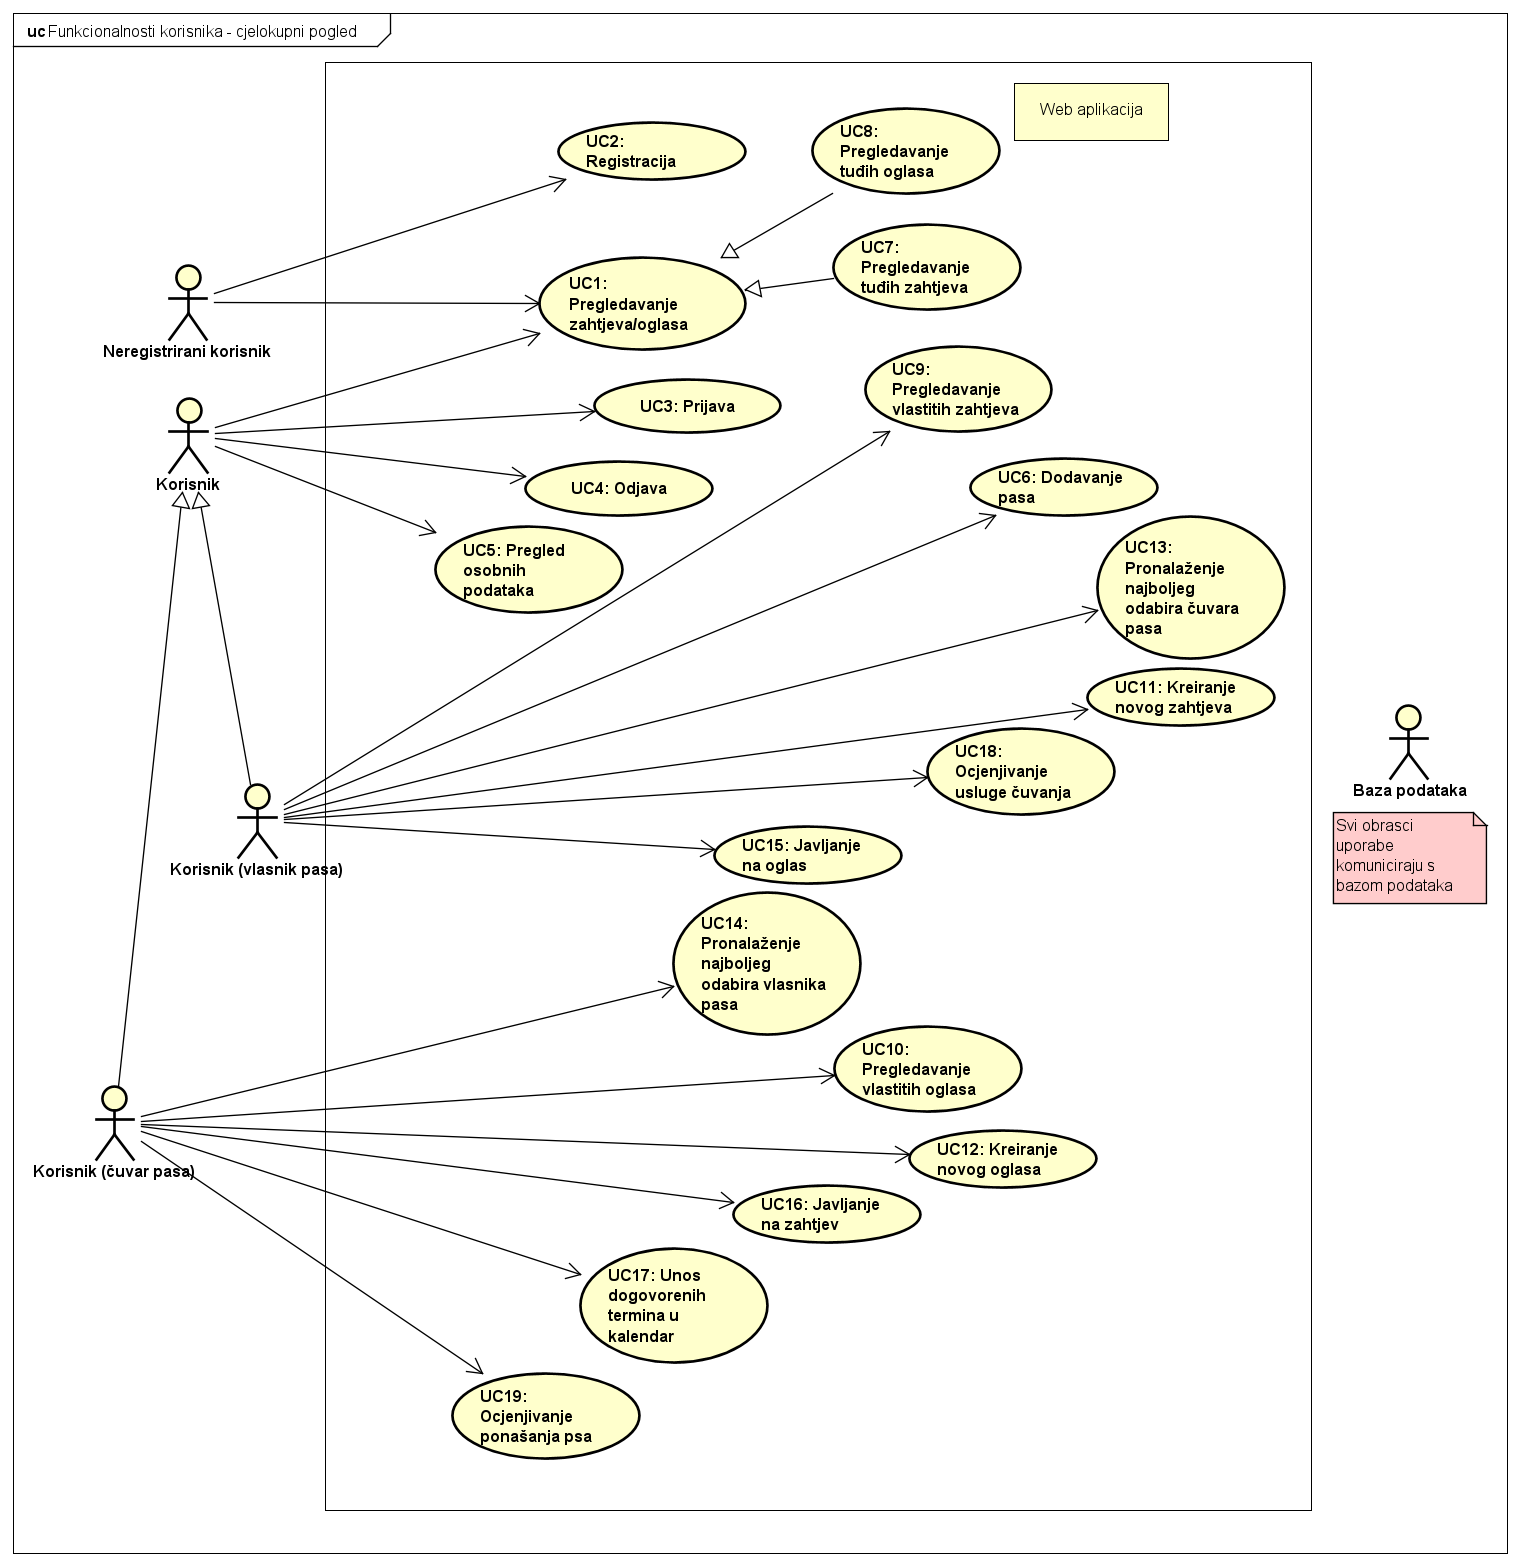
\includegraphics[width=12cm]{slike/korisnikExport}
						\caption{Dijagram obrasca uporabe, funkcionalnost neregistriranog korisnika i korisnika (vlasnika pasa i čuvara pasa)}
						\label{fig:DOU-korisnici}
					\end{figure}
				\eject		
					\begin{figure}[htb]
						\centering
						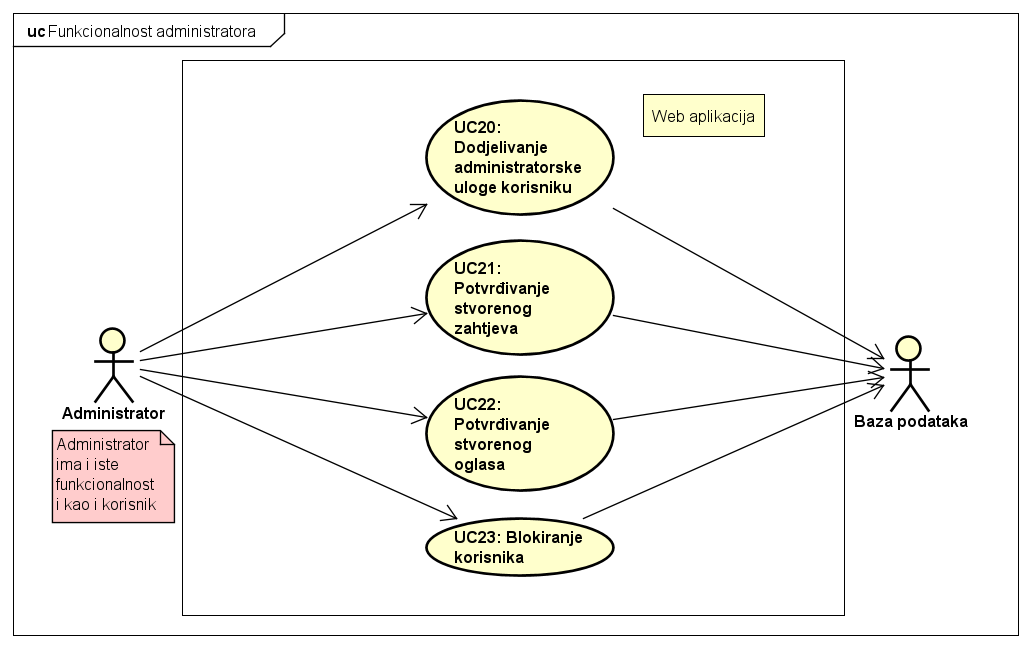
\includegraphics[width=12cm]{slike/dijagramExport}
						\caption{Dijagram obrasca uporabe, funkcionalnost administratora}
						\label{fig:DOU-administrator}
					\end{figure}
				\eject		
				
			\subsection{Sekvencijski dijagrami}
				
				\textbf{Obrazac uporabe UC11 - Kreiranje novog zahtjeva}\\
				
				Korisnik (vlasnik pasa) na početnoj stranici odabire opciju za kreiranje novog zahtjeva. Web aplikacija mu otvara stranicu za kreiranje zahtjeva. Korisnik tamo unosi tražene podatke (pasmina, dob, period čuvanja, itd.) za kreiranje zahtjeva. Potom korisnik potvrđuje kreiranje zahtjeva. Ako korisnik nije ispravno unio podatke, prilikom potvrde web aplikacija ga ponovno usmjerava na istu stranicu s prikladnom porukom o greški. Web aplikacija mu daje odgovor o uspješnom kreiranju zahtjeva. Zahtjev se pohranjuje u bazu podataka.
				
				\begin{figure}[htb]
					\centering
					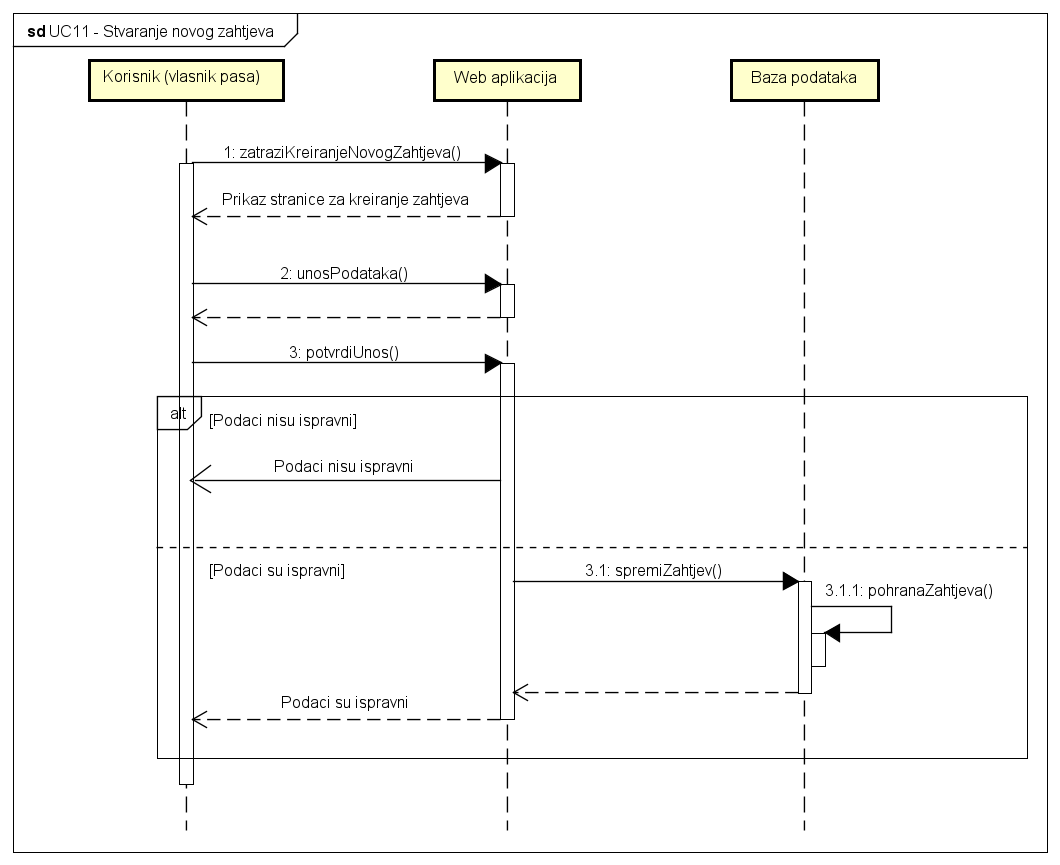
\includegraphics[width=16cm]{slike/UC11 - Stvaranje novog zahtjeva - sekvencijski - v3}
					\caption{Sekvencijski dijagram za UC11}
					\label{fig:Sekvencijski-UC11}
				\end{figure}
				\eject		
				
				\textbf{Obrazac uporabe UC14 - Pronalaženje najboljeg odabira vlasnika pasa}\\
				
				Korisnik (čuvar pasa) na početnoj stranici odabire opciju "Moji oglasi". Web aplikacija mu otvara stranicu s njegovim oglasima. Korisnik tamo pokraj željenog oglasa pritišće gumb "Pronalaženje najboljeg odabira". Web aplikacija pronalazi najboljeg vlasnika pasa i šalje ga korisniku. Korisnik ima mogućnost ga prihvatiti, ali i odbiti. Ako korisnik odbije, nema daljnje suradnje s vlasnikom pasa. Ako ga korisnik prihvati, obavijest se šalje vlasniku pasa da je došlo do najboljeg odabira. Tamo vlasnik pasa ima također opciju prihvatiti suradnju kao i odbiti ju.
				
				\begin{figure}[htb]
					\centering
					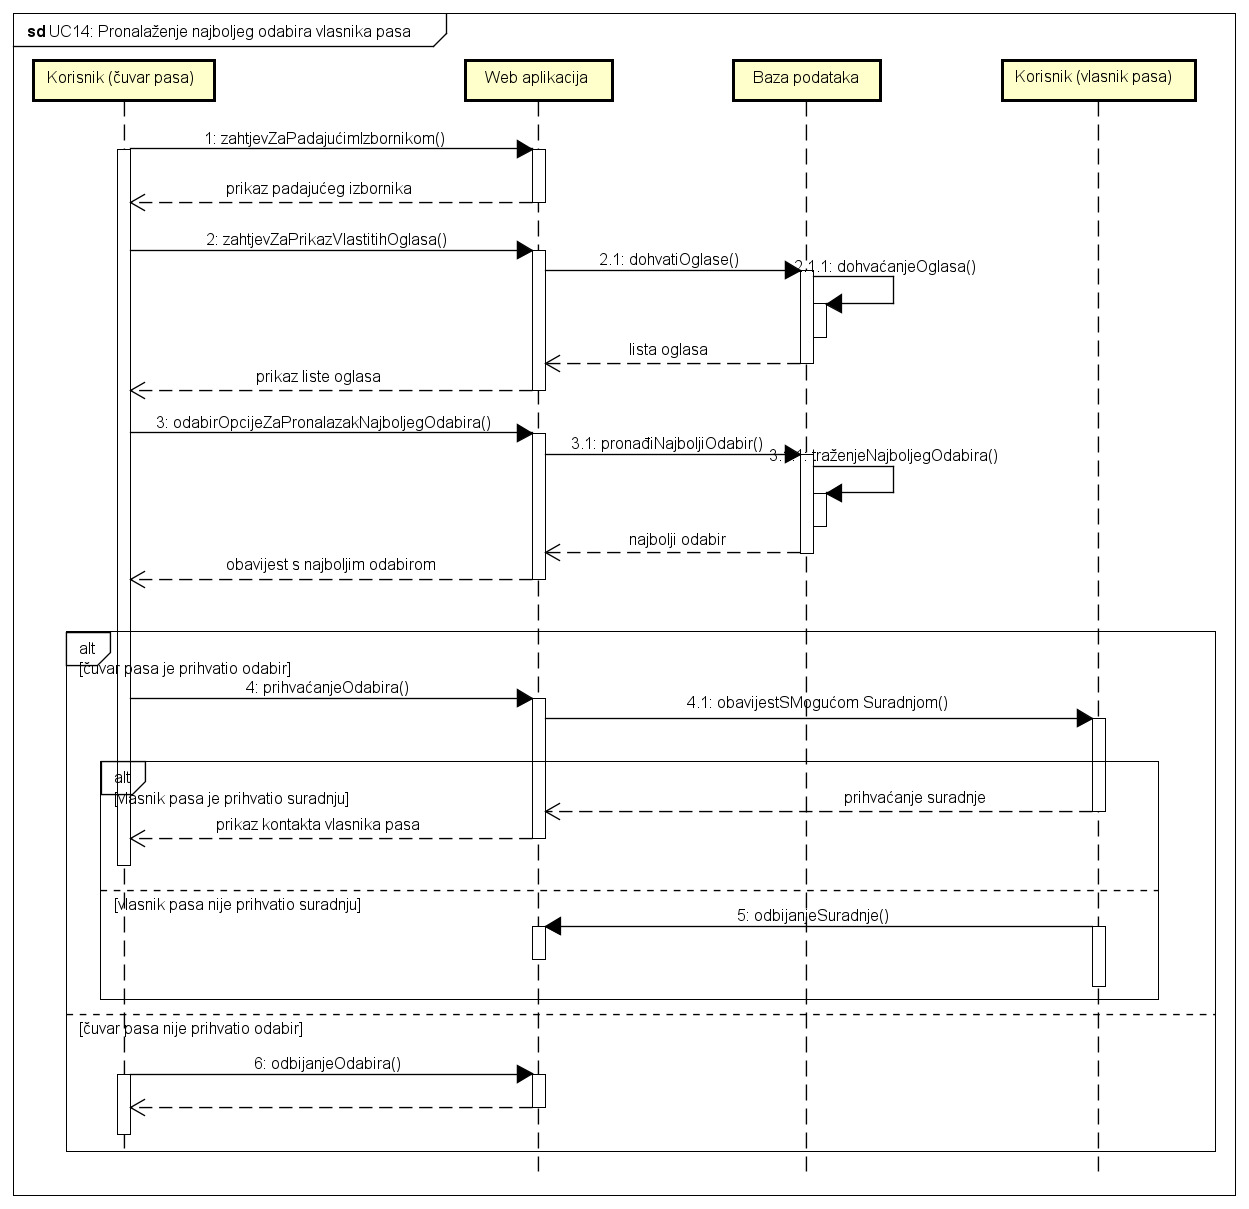
\includegraphics[width=16cm]{slike/UC14 - sekvencijski}
					\caption{Sekvencijski dijagram za UC14}
					\label{fig:Sekvencijski-UC14}
				\end{figure}
				\eject		
				
				\textbf{Obrazac uporabe UC21 - Potvrđivanje stvorenog zahtjeva}\\
				
				Administrator sustava na početnoj stranici odabire opciju za pristupanje stranici za administratorsko upravljanje. Web aplikacija šalje upit za potrebnim elementima (svi nepotvrđeni zahtjevi i oglasi te svi korisnici sustava) bazi podataka. Primitkom istih, web aplikacija otvara stranicu administratoru. Administrator u listi zahtjeva pronalazi željeni zahtjev te kraj njega pritišće gumb za njegove potvrđivanje. Web aplikacija šalje upit za ažuriranjem zahtjeva bazi podataka. Baza podataka ga ažurira i šalje ažuriranu listu zahtjeva web aplikaciji. Web aplikacija otvara ponvono stranicu administratoru, ali sada s ažuriranom listom zahtjeva.
				
				\begin{figure}[htb]
					\centering
					\includegraphics[width=16cm]{slike/UC21 - Potvrđivanje stvorenog zahtjeva - sekvencijski}
					\caption{Sekvencijski dijagram za UC21}
					\label{fig:Sekvencijski-UC21}
				\end{figure}
				\eject	
				
				\textbf{Obrazac uporabe UC23 - Blokiranje korisnika}\\
				Administrator sustava na početnoj stranici odabire opciju za pristupanje stranici za administratorsko upravljanje. Web aplikacija šalje upit za potrebnim elementima (svi nepotvrđeni zahtjevi i oglasi te svi korisnici sustava) bazi podataka. Primitkom istih, web aplikacija otvara stranicu administratoru. Administrator u listi korisnika pronalazi željenog korisnika te kraj njega pritišće gumb na njegovo blokiranje. Web aplikacija šalje upit za brisanjem korisnika u bazi podataka. Baza podataka briše korisnika i šalje ažurirana listu korisnika web aplikaciji. Web aplikacija otvara ponovno stranicu administratoru, ali sada s ažuriranom listom korisnika.
				
				\begin{figure}[htb]
					\centering
					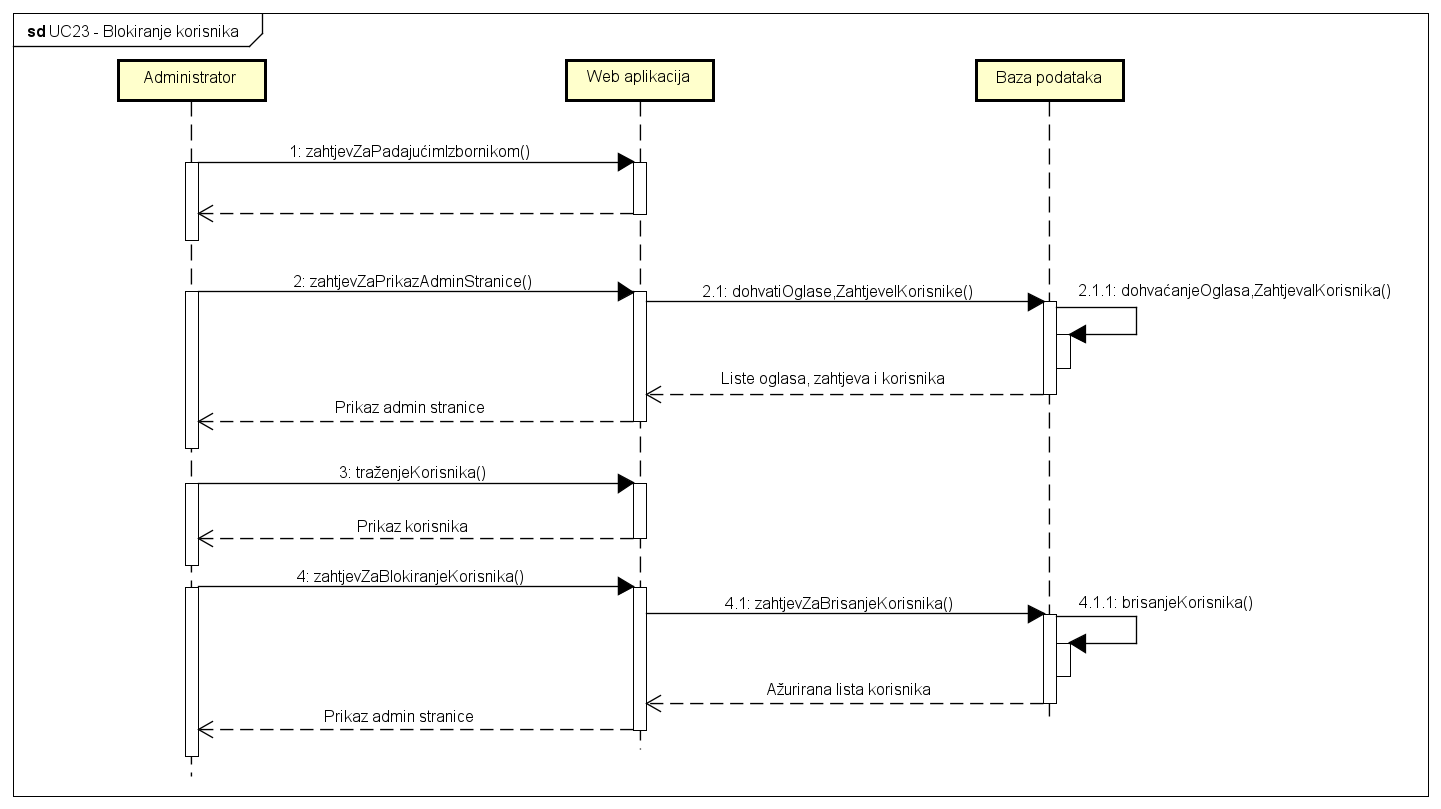
\includegraphics[width=16cm]{slike/UC23 - Blokiranje korisnika - sekvencijski}
					\caption{Sekvencijski dijagram za UC23}
					\label{fig:Sekvencijski-UC23}
				\end{figure}
				\eject	
	
		\section{Ostali zahtjevi}
		
			\begin{packed_item}
				
				\item Aplikacija treba biti izvedena kao web aplikacija prilagođena mobilnom uređaju i tabletu
				\item Aplikaciji pristupaju registrirani korisnici uz pomoć korisničkog imena i lozinke
				\item Sustav treba podržavati rad više korisnika u stvarnom vremenu
				\item Aplikaciju treba implementirati u arhitekturi klijent-poslužitelj
				\item Na poslužiteljskoj strani se treba koristit programski jezik Java i radni okvir Spring Boot
				\item Podaci se trebaju spremati u relacijsku bazu podataka koristeći JPA
				\item Funkcionalnost web aplikacije se treba izložiti kroz REST Web servis
				\item Na klijentkoj strani treba implementirati korisničko sučelje u Web pregledniku koristeći React, koje se spaja na navedene servise
			\end{packed_item}
			 
			 
			 
	